\documentclass[a4paper,11pt]{report}

\usepackage[utf8]{inputenc}
\usepackage[ngerman]{babel}
\usepackage[T1]{fontenc}
\usepackage{graphicx}
\usepackage{amsmath}
\usepackage{amssymb}
\usepackage{float}
\usepackage[format=hang]{caption}


\title{Dissertation}
\author{Heiner Kolp}

\begin{document}

\setlength{\parindent}{0pt}
\maketitle
\tableofcontents

\chapter{Einleitung}

\section{Epilepsie}
Epilepsie ist eine Erkrankung des Gehirns die durch eine anhaltende Prädisposition gegenüber epileptischen Anfällen ausgezeichnet ist und die mit neurobiologischen, kognitiven, psychologischen und sozialen Konsequenzen einher geht. Ein epileptischer Anfall ist definiert als vorübergehendes Auftreten von Zeichen und/oder Symptomen aufgrund abnormer exzessiver oder synchroner neuronaler Aktivität im Gehirn.\cite{Fisher.2005}\\
Eine der ersten dokumentierten medikamentösen Therapien im 19. Jahrhundert war die mit Natriumbromid {\cite{OConnor.1857}\cite{ToddRobertBentley18091860.}. Als offizieller Begründer der medikamentösen Therapie wird Charles Locock betitelt \cite{Brodie.2010}. Als damaliger Präsident der Royal Medical and Chirurgical Society kommentierte er 1857 den Artikel seines Kollegen E.H. Sieveking \cite{Sieveking.1857} und verwies auf seine Erfolge mit Bromid \cite{Eadie.2012}.\\
Der Erste Durchbruch gelang 1912 dem deutschen Neurologen Alfred Hauptmann mit der Verwendung von Phenobarbital. \cite{Hauptmann.1912}. Besonders bemerkenswert ist die Tatsache, dass Phenobarbital bis heute zu den gängigen Medikamenten bei Epilepsien sowohl im Kindes-, als auch Erwachsenenalter zählt.\cite{DGN.2017} Für die nächsten 30 Jahre dominierten Bromid und PB die Therapieregime. Bromid behielt vor allem wegen der langjährigen Erfahrung die Position als Mittel der Wahl, auch wenn PB immer mehr durch die Reduktion der psychomotirschen Verlangsamung und anderer neurologischer Nebenwirkungen von Bromid an Bedeutung gewann. \cite{Yasiry.2012}\\
Ein Rückgang der Therapie mit Bromid kündigte sich erst 1940 mit der Entdeckung von Phenytoin \cite{Merritt.1938}an.
\chapter{Material und Methoden}

\section{Chemikalien und Lösungen}

\subsection{Verwendete Chemikalien}

\subsection{Herstellen der Lösungen}

\section{Geräte}

\section{Versuchstiere}
Alle Experimente wurden an männlichen Wistar-Ratten (Charles River Laboratories GmbH, Sulzfeld, Deutschland; XXXXXXXXXXXXXXX) durchgeführt. Die Tiere wurden vor dem  achten Lebenstag in Gruppen von 12 bis 15 Jungtieren und einer Mutter geliefert. Dann erfolgte die Haltung bei stabilen klimatischen Bedingungen und einem festgelegten Hell-Dunkel-Zyklus mit 12 Stunden Belichtung und Nahrung und Wasser ad libitum. Die Trennung der Tiere von der Mutter erfolgte an Tag XX zu Paaren. Ab Tag XX erfolgte die Einzelhaltung.
\section{Methoden}
Alle angewandten experimentellen Verfahren entsprachen nationalen und internationalen Richtlinien bzgl. der ethischen Verwendung von Tieren (European Council Directive 86/609/EEC).
\subsection{Pilokarpininjektion}
Am Tag der Injektion wurden alle Jungtiere gegen 9 Uhr aus dem Stall in den Tierversuchsraum gebracht und dort von der Mutter getrennt. Anschließend wurden die Tiere gewogen. Die leichtesten  zwei Tiere wurden zurück zur Mutter gesetzt. Die Mutter mit den beiden Jungtieren wurde für die Dauer der Injektion zurück in den Tierstall gebracht.  Für die übrigen Tiere erfolgte eine zufällige Aufteilung entweder zur Versuchsgruppe oder zur Kontrollgruppe.  Für die Dauer der Injektion befanden sich alle Tiere in einem Sammelkäfig. Dieser wurde mit einer Heizmatte und einer Rotlichtlampe beheizt. Die beiden Gruppen wurden für die eindeutige Zuordnung während der Injektionen farblich unterschiedlich nummeriert. \\

Um die peripheren cholinergen Wirkungen des Pilokarpins zu reduzieren wurden alle Tiere mit N-Methylscopolamin-Lösung 100$\mu l$ pro 20$g$ Körpergewicht i.p. injiziert. 30 Minuten später erfolgte für die Versuchstiere die Injektion mit Pilokarpin-Lösung 100$\mu l$ pro 20$g$ Körpergewicht i.p. Kontrolltiere wurden analog mit 100$\mu l$ NaCl-Lösung injiziert.\\

40 Minuten nachdem das erste Tier einen SE entwickelt hatte, wurde dieser bei allen Versuchstieren mit Diazepam terminiert. Es ist zu bemerken, dass die Entwicklung eines SE bei allen Tieren in einem Zeitraum von fünf bis zehn Minuten nach der Pilokarpininjektoin erfolgte. Es wurde alle Tieren 10-30$\mu l$ Diazepam-Lösung injiziert. Die Dosierung erfolgte abgestimmt auf die Ausprägung des SE und der Anfälle während des SE. Bei Bedarf wurden 10$\mu l$ Diazepam nachgegeben. Direkt nach der Injektion, bevor eine Wirkung eintreten konnte, wurde allen Tieren frisch angesetzte Glukoselösung mit einer Pipette angeboten. Sobald die Tiere schliefen, wurden ihnen zum Ausgleich von Flüssigkeitsverlusten 200$\mu l$ NaCl-Lösung s.c. verabreicht. Nach 60 Minuten erfolgte eine zweite Gabe von NaCl-Lösung s.c. \\

Nach der zweiten Gabe von NaCl-Lösung wurden alle Tiere zurück zur Mutter gegeben.
Am ersten Injektionstag wurden alle Tiere während der Schlafphase nach Injektion des Diazepams eindeutig an den Pfoten tätowiert. An den folgenden Tagen wurden die Tätowierungen kontrolliert und gegebenenfalls erneuert. \\

\subsection{Präparation der Hirnschnitte}
Die Präparation der Hirnschnitte erfolgte immer nach demselben festgelegten Schema um eine gleichbleibende Qualität zu sichern.\\
Zunächst erfolgte eine tiefe Diethylether-Narkose, welche durch einen Schmerzreiz und die dabei ausbleibende Reaktion des Tieres kontrolliert wurde. Bei ausreichend tiefer Narkose erfolgte die Dekapitation mithilfe einer Guillotine. Der abgetrennte Kopf wurde sofort in einen zuvor bereitgestelltes breitbasiges Behältnis gelegt, in dem sich mit Carbogen (95$\%$ $CO_2$, 5$\%$ $O_2$) eisgekühlte Succrose-Lösung befand. Die weitere Präparation erfolgte in jenem Gefäß. Der nächste Schritt war eine mediane Inzisur der Kopfhaut mit einem Skalpell mit der der Schädelknochen freigelegt wurde. Anschließend erfolgte mit einer schmalschneidigen Schere die Eröffnung des Schädels vom Foramen magnum aus nach kranial bis hin zum Bregma. Hierbei wurde idealerweise auch die harte Hinrhaut (Dura mater) bereits aufgetrennt. Nach zwei lateralen Schnitten zur Durchtrennung des Os occipitale am Foramen magnum konnte die Schädeldecke mithilfe einer Pinzette vorsichtig zur Seite aufgeklappt werden. Mit einem Skalpell wurde das Kleinhirn (Cerebellum) und Teile des Hirnstamms entfernt. Durch einen gebogenen Spatel konnte nun das verbleibende Gehirn entfernt und in ein sauberes, mit eisgekühlter, durch Carbogen begaster Succrose gefülltes Transportgefäß gegeben werden. Zwischen Dekapitierung und Einfügen in das Transportgefäß sollten nie mehr als 60 Sekunden vergehen. 

Im Anschluss wurde das Gehirn mit handelsüblichem Sekundenkleber auf dem Schnittblock der Schnittkammer so fixiert, dass die occipitale Seite des Gehirns zur Schneidklinge und die Unterseite der Temporallappen nach oben wiesen. Sobald das Gehirn aufgebracht war, wurde die Schnittkammer mit eisgekühlter Succrose-Lösung befüllt und mit Carbogen begast. Daraufhin wurden mit dem Vibratom 400$\mu m$ Dicke Schnitte bei einem Vortrieb von 0,6$mm$ pro Sekunde im Bereich des Hippocampus angefertigt. Die Region des Hippocampus wurde dann auf der Klinge liegend abgetrennt und mit einer Transferpipette in die Aufbewahrungskammer überführt. 

\subsection{Elektrophysiologiesche Messungen} 

Um möglichst störfreie und adäquate elektrophysiologische Messungen durchzuführen, befand sich der Messplatz in einem faradayschen Käfig auf einem vibrationsgedämpften Tisch. Oberhalb der Messkammer befand sich ein Stereomikroskop mit einer Kaltlichtquelle zur genauen Positionierung der Elektroden.\\

Bis zu zwei Hirnschnitte ruhte in der Messkammer auf einem Nylonnetz, umspült von mit Carbogen begaster Messlösung und bei durch einen Temperaturregler konstant gehaltener Temperatur von $32^\circ C \pm 1^\circ C$ . Die Flussrate wurde dabei durch eine Rollerpumpe konstant gehalten. Nach Einbringen der Schnitte in die Messkammer wurde immer eine Inkubationszeit von mindestens 20 Minuten abgewartet, bevor Messungen durchgeführt wurden.\\

Für Feldpotentialmessungen befanden sich zu beiden Seiten der Messkammer jeweils eine Stimulations- und eine Ableitelektrode, montiert auf einem Mikromanipulator. Die eigentliche Elektrode bestand aus einem chlorierten Silberdraht in einer mit Messlösung gefüllten Boroselikatpipette mit einem Spitzenwiderstand von 2-3 $M\Omega$. Die Stimulationselektroden waren mit einem Impulsgenerator verbunden, welcher über einen Frequenzregulator kontrolliert wurde. Die Ableitelektroden gaben über einen Vor- und einen Hauptverstärker ihr Signal an einen Stromwandler, welcher die Information weiter an einen Rechner gab.\\

Für die Intrazellulären Messungen befand sich auf der einen Seite der Messkammer eine Stimulationselektrode, analog zu den Feldpotentialmessungen. Auf der anderen Seite befand sich die intrazelluläre Elektrode auf einem schrittmotorgetriebenen Mikromanipulator. Sie bestand aus einem dünnem chloriertem Silberdraht, der in eine mit intrazellulärer Lösung befüllte Glaspipette eingebracht war. Die intrazelluläre Elektrode war ebenfalls über einen Vor- und einen Hauptverstärker, und einen Stromwandler mit einem Rechner verbunden.\\

Am Rechner erfolgte die Darstellung und Bearbeitung der Ableitungen über das Programm Signal 2.16. Ebenso war es uns mithilfe von Signal umgekehrt möglich die Zelle intrazellulär mit verschiedenen Stromprotokollen zu erregen.\\

Die Speicherung der Daten erfolgte am Ende in digitaler Form auf Speichermedien.\\

Bei der Auswertung der Daten benutze ich den Begriff Baseline. In dieser Arbeit definiere ich ihn als den Zeitraum des Beginns einer Messung in dem sich die Hirnschnitte in relativer Ruhe befinden. Am Beispiel der Feldpotentialmessungen sind es die ersten 20 Minuten vom Beginn der Messung bis zur HFS. 

\subsubsection{Ziehen von Pipetten}

\subsubsection{Feldpotentialmessungen}

\subsubsection{Intrazelluläre Messungen}

\chapter{Ergebnisse}
\section{Einfluss von Bromid auf die Langzeitpotenzierung}
Die Anwendung eines Hochfrequenzstimulationsprotokolls an Zellen der CA1-Region des Hippocampus  löst üblicherweise eine Langzeitpotenzierung der synaptischen Antworten aus. Zu Beginn  jeder Aufnahme werden bei halbmaximaler Stimulationsstärke stabile fEPSP über einen Zeitraum von$20\, min$ gemessen um das Ausgangsniveau festzustellen. Anschließend wird eine HFS ($100\,Hz$ für $1\,s$) bei maximaler Stimulationsstärke durchgeführt. Die Auswirkung der HFS wird für $60\, min$ bei wiederum halbmaximaler Stimulationsstärke gemessen um eine mögliche LTP zu erfassen.

Für Versuche unter therapeutischen Bedingungen wurden  $20\, mmol$ NaCl der Nährlösung ACSF isoosmolar durch NaBr substituiert.\\

 Diese Hochfrequenzstimulation führt bei Hippocampusschnitten von unbehandelten Tieren ohne NaBr zu einer kurzfristig starken Erhöhung der fEPSP-Amplitude, die im Verlauf der nächsten $60\, min$ auf einen stabilen Wert von $110\,\pm 5\,\%$ des Ausgangsniveaus absinkt.
 %110,80 \pm 5,35

\begin{figure}[H]
\begin{center}
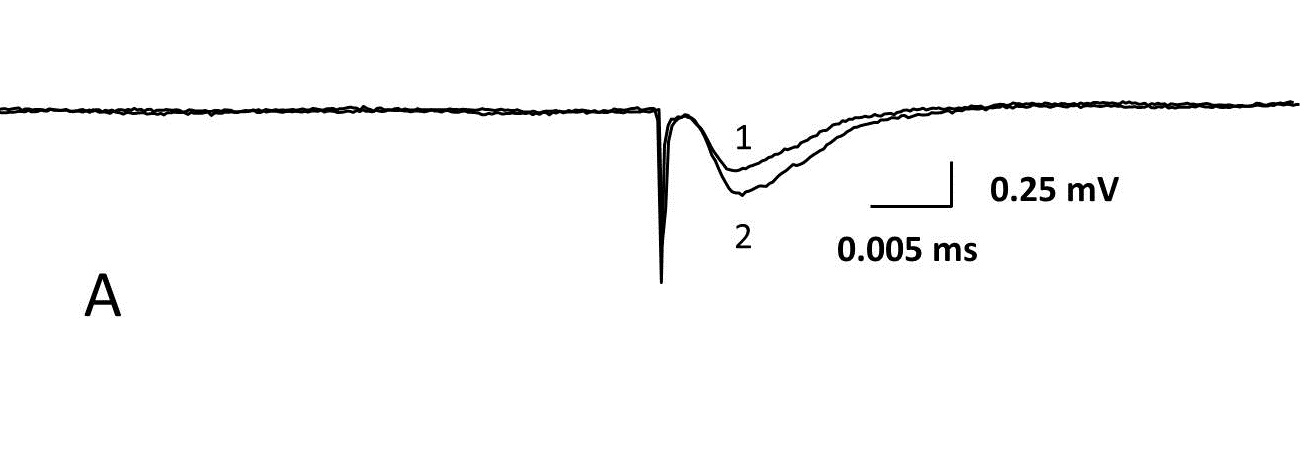
\includegraphics[width=6cm]{Abbildungen/feld_samples/field_k_c.jpg}
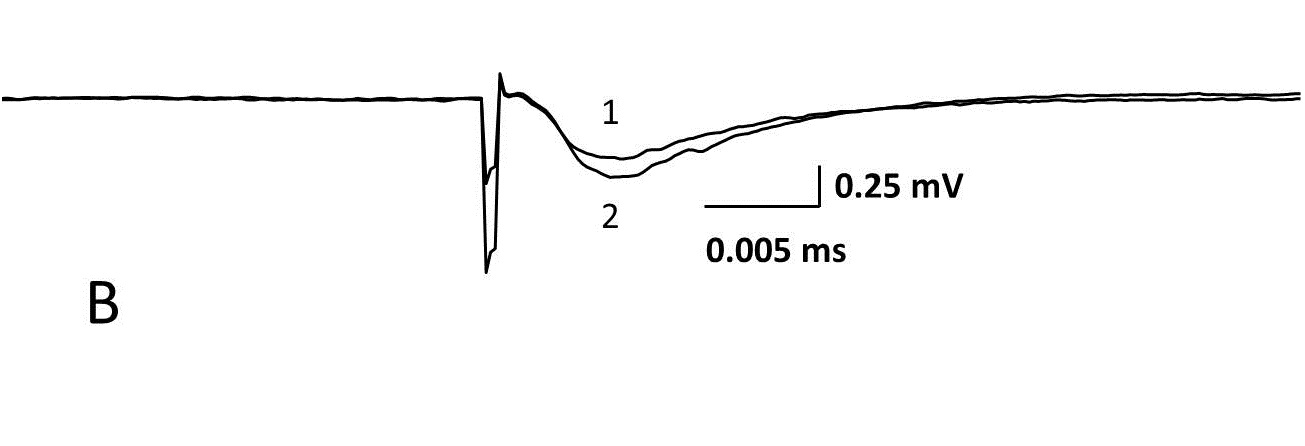
\includegraphics[width=6cm]{Abbildungen/feld_samples/field_k_br.jpg}
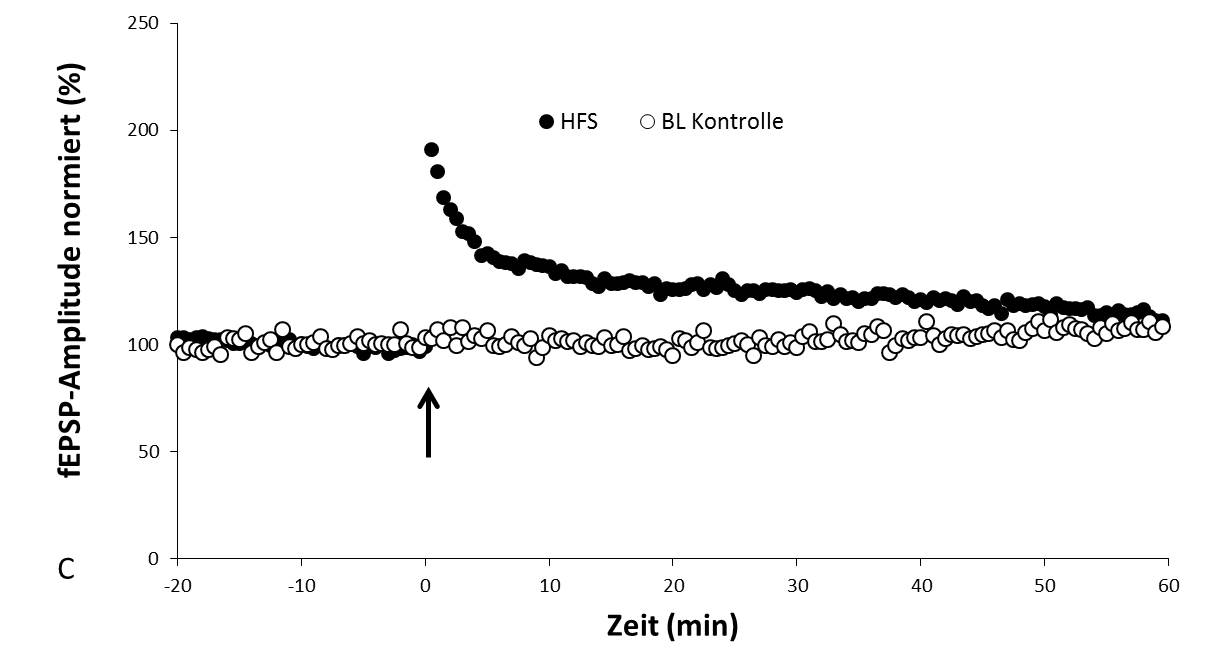
\includegraphics[width=13cm]{Abbildungen/feld_samples/ltp_k_chfs_mean}
\caption{Repräsentative Originalaufzeichnungen von Feldpotentialmessungen an Hippocampusschnitten von unbehandelten Tieren. \textbf{A} zeigt exzitatorische postsynaptische Potentiale  für eine Einzelstimulation im Feld (fEPSP) während der Registrierung des Ausgangsniveaus (1) und am Ende der Registrierung nach Hochfrequenzstimulation (2) in ACSF Nährlösung. \textbf{B} analog unter Verwendung einer modifizierten Nährlösung. In dieser sind $20\, mmol$ NaCl isoosmolar durch NaBr substituiert. \textbf{C} fEPSP-Amplituden normiert auf den Mittelwert der Ausgangsregistrierung. Während der durch die ausgefüllten Symbole dargestellten Messung wird zum Zeitpunkt Null (Pfeil)die Hochfrequenzstimulation durchgeführt wird. Die geschlossenen Symbole zeigen den Verlauf einer Kontrollmessung ohne Hochfrequenzstimulation.}
\end{center}
\end{figure}


Die Verwendung der modifizierten Nährlösung ACSF/Br führt zu einer Erhöhung der fEPSP-Amplitude auf $113\,\pm 7\,\%$ der Ausgangswerte. Damit  unterscheiden sich diese beiden Gruppen nicht signifikant.\\
%113,48 \pm 7,75
Die HFS an Hippocampusschnitten von mit Pilocarpin behandelten Tieren führt zu einem Anstieg der fEPSP-Amplituden auf $126\,\pm 9\,\%$. Die isoosmolare Substitution  von$20\, mmol$ NaCl mit NaBr vermindert diesen Anstieg auf $114\,\pm 7\,\%$. Der Unterschied hierbei ist jedoch statistisch nicht signifikant (Mann-Withney-U-Test).\\
%126,34 \pm 9,24
%114,06 \pm 7,72
Für beide Versuche wurde durch Kontrollen ohne HFS gezeigt, dass die fEPSP-Amplitude das Ausgangsniveau beibehält.\

In den Abbildungen 3.1 und 3.2 sind beispielhaft fEPSPs für die verschiedenen Gruppen dargestellt. Abbildung 3.3 vergleicht die LTP-Werte der einzelnen Gruppen grafisch.



\begin{figure}
\begin{center}
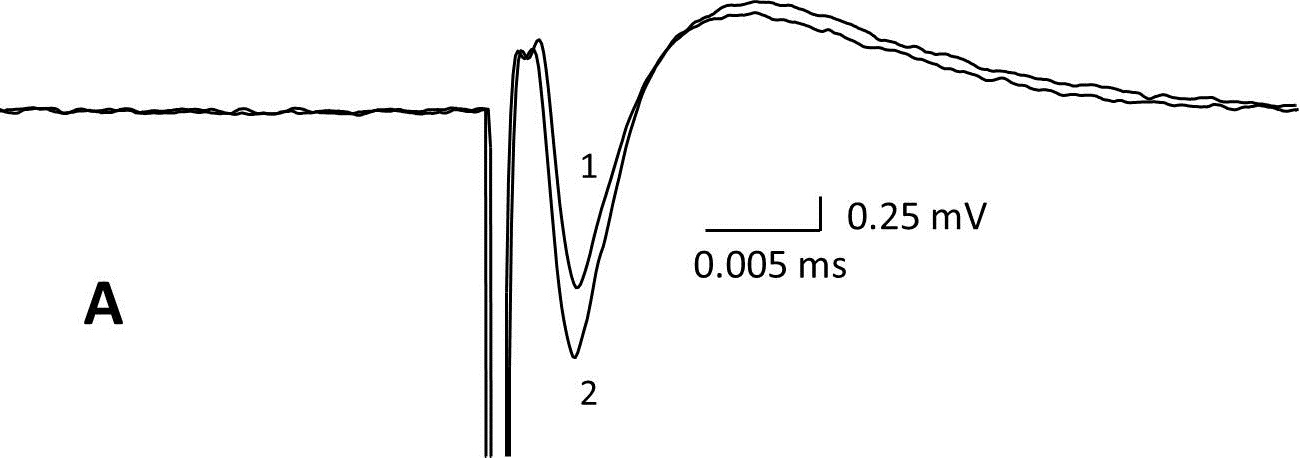
\includegraphics[width=6cm]{Abbildungen/feld_samples/field_p_c}
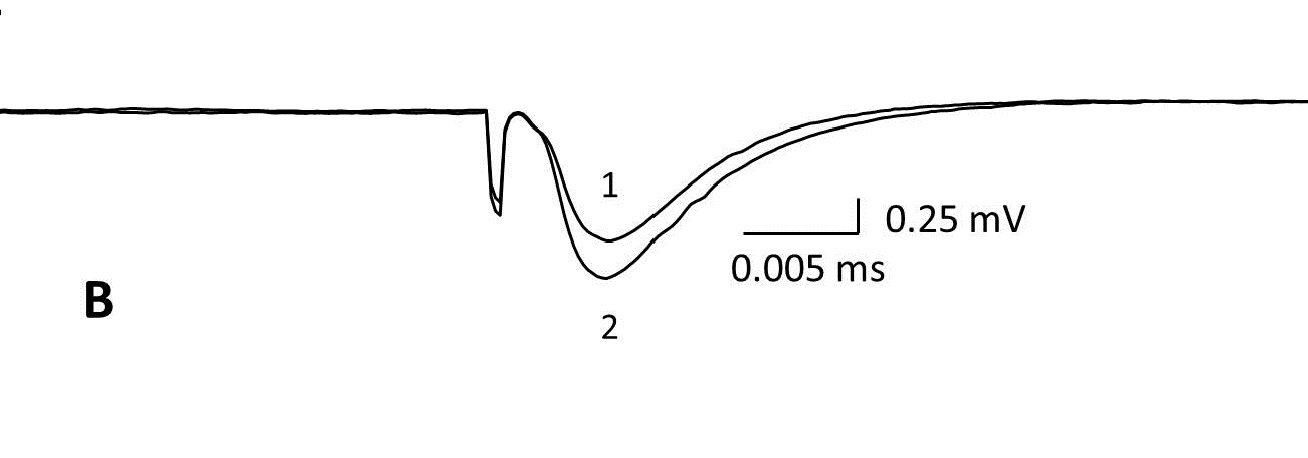
\includegraphics[width=6cm]{Abbildungen/feld_samples/field_p_br}
\caption{Repräsentative Originalregistrierungen von Feldpotentialmessungen an Hippocampusschnitten von mit Pilocarpin behandelten Tieren. Zeitpunkt (1) ist während der Registrierung des Ausgangsniveaus, Zeitpunkt (2) am Ende der Registrierung nach Hochfrequenzstimulation. \textbf{A} Stellt eine Messung mit  ACSF als Nährlösung dar, \textbf{B} eine Messung unter Verwendung von ACSF/Br. Diese unterscheiden sich durch die isoosmolare Substitution von $20\, mmol$ NaCl durch NaBr.}
\end{center}
\end{figure}

\begin{figure}[H]
\begin{center}
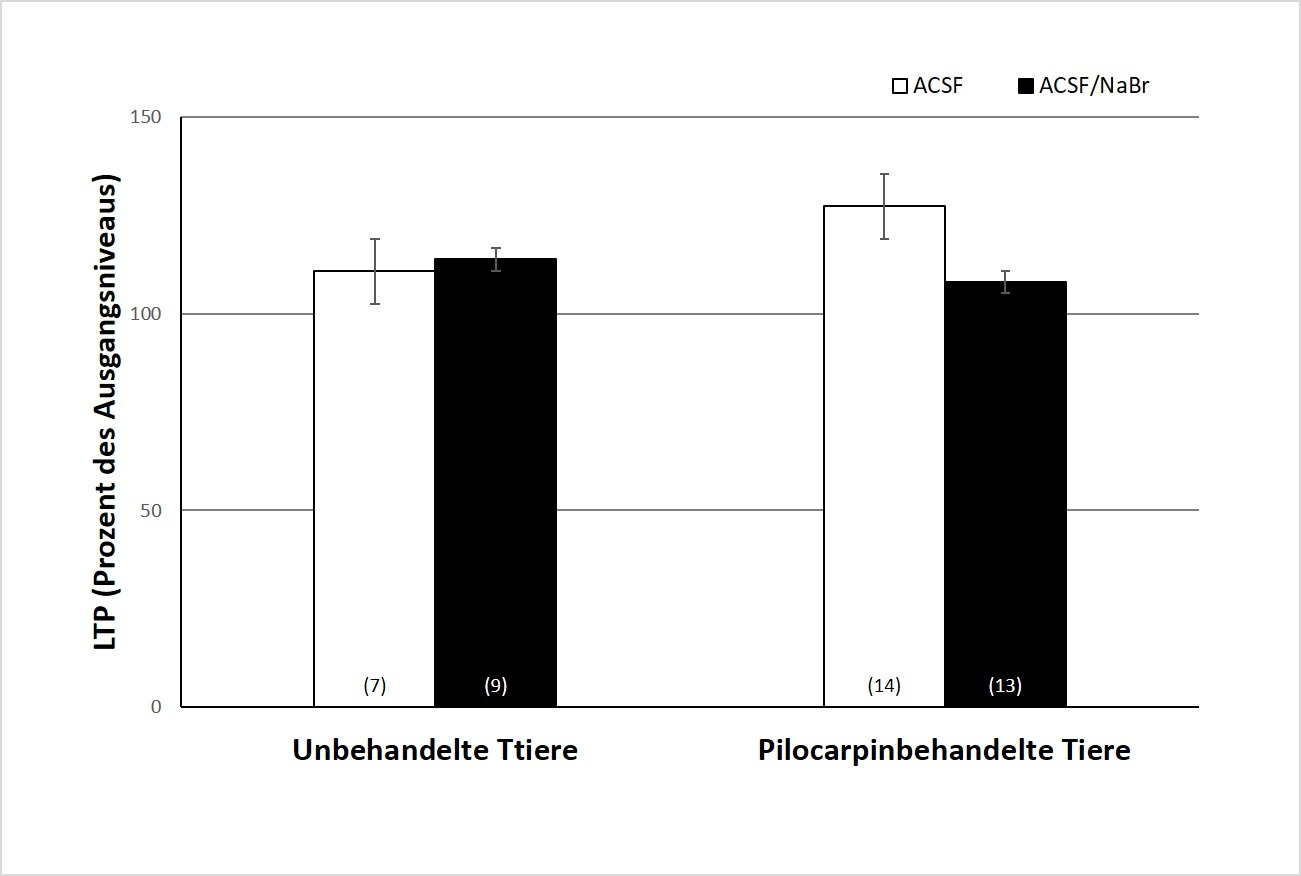
\includegraphics[width=13cm]{Abbildungen/feld_samples/ltp_diagramm.jpg}
\caption{Vergleich der Langzeitpotenzierung (Prozent des Ausgangsniveaus) $60\,min$ nach Hochfrequenzstimulation mit Darstellung des Standardfehlers und Angabe der Anzahl der verwendeten Präparate (Zahlen in Klammern). Bei Präparaten von unbehandelten Tieren gibt es keinen Unterschied zwischen der Verwendung von herkömmlicher Nährlösung ACSF und der modifizierten Nährlösung ACSF/NaBr, welche NaBr enthält. Wenngleich die Langzeitpotenzierung bei mit Pilocarpin behandelten Tieren unter Verwendung von ACSF im Mittel erhöht ist, unterscheiden sich auch diese Werte nicht signifikant von den anderen Gruppen. In der mit NaBr behandelten Gruppe der mit Pilocarpin behandelten Tiere liegt die Langzeitpotenzierung auf dem Niveau der unbehandelten Tiere. Insgesamt wurden Messungen an Hippocampusschnitten von sechs unbehandelten Tieren und zwölf mit Pilokarpin behandelten Tieren verwendet.}  
\end{center}
\end{figure}

\section{Charakterisierung der Membraneigenschaften}

Nach Bestimmung der synaptischen Plastizität wurden die Membraneigenschaften einzelner Zellen charakterisiert. Hierzu wurden Pyramidenzellen der CA1-Region mit Hilfe von scharfen Mikroelektroden sogenannten sharp micro electrodes identifiziert und durch einen Haltestrom auf einem Membranpotential bei $-70\,mV$ stabilisiert. Die Zellen zeigten während einer Zeit von $10\,min$  ein stabiles Verhalten, bevor sie gemessen wurden. Ohne den Haltestrom musste jede Zelle ein Ruhemembranpotential von $-55\,mV$ oder negativer aufweisen. Durch intrazelluläre Strominjektionen in Höhe von $-1.3$ $nA$ bis $+1.4$ $nA$ (in Schritten von $0.1$ $nA$) wurden Strom-Spannungs-Relationen gemessen und für die Berechnung der Membraneigenschaften genutzt. \\



%Der Membranwiderstand der Zellen von Kontrolltieren ohne Beigabe von NaBr ist im Mittelwert $47,54 \pm 7,44M\Omega$. Der Mittelwert bei Zugabe von NaBr Hirnschnitten liegt bei $53,10 \pm 5,96M\Omega$.



%Die Untersuchungen bei Pilo-Tieren ergeben für Messungen ohne NaBr einen mittleren Membranwiderstand von $36,22 \pm 1,74 M\Omega$. Bei Zugabe von NaBr ergibt sich ein Mittelwert von $31,52 \pm 3,07 M\Omega$. Die beiden Mittelwerte unterscheiden sich nicht signifikant voneinander.\\

Die Ergebnisse der Charakterisierung der Membraneigenschaften sind in Tabelle 3.1 zusammenfassend dargestellt. Im Ganzen ergaben sich zwei signifikante Unterschiede: die Membranzeitkonstante wurde durch die Verwendung der modifizierten Nährlösung ACSF/NaBr in der Gruppe der pilocarpinbehandelten Tiere erhöht; in der Gruppe der unbehandelten Tiere erhöhte sich das Potenzial der Nachhyperpolarisation AHP unter Verwendung der modifizierten Nährlösung ACSF/NaBr.

\begin{table}[H]
\begin{center}
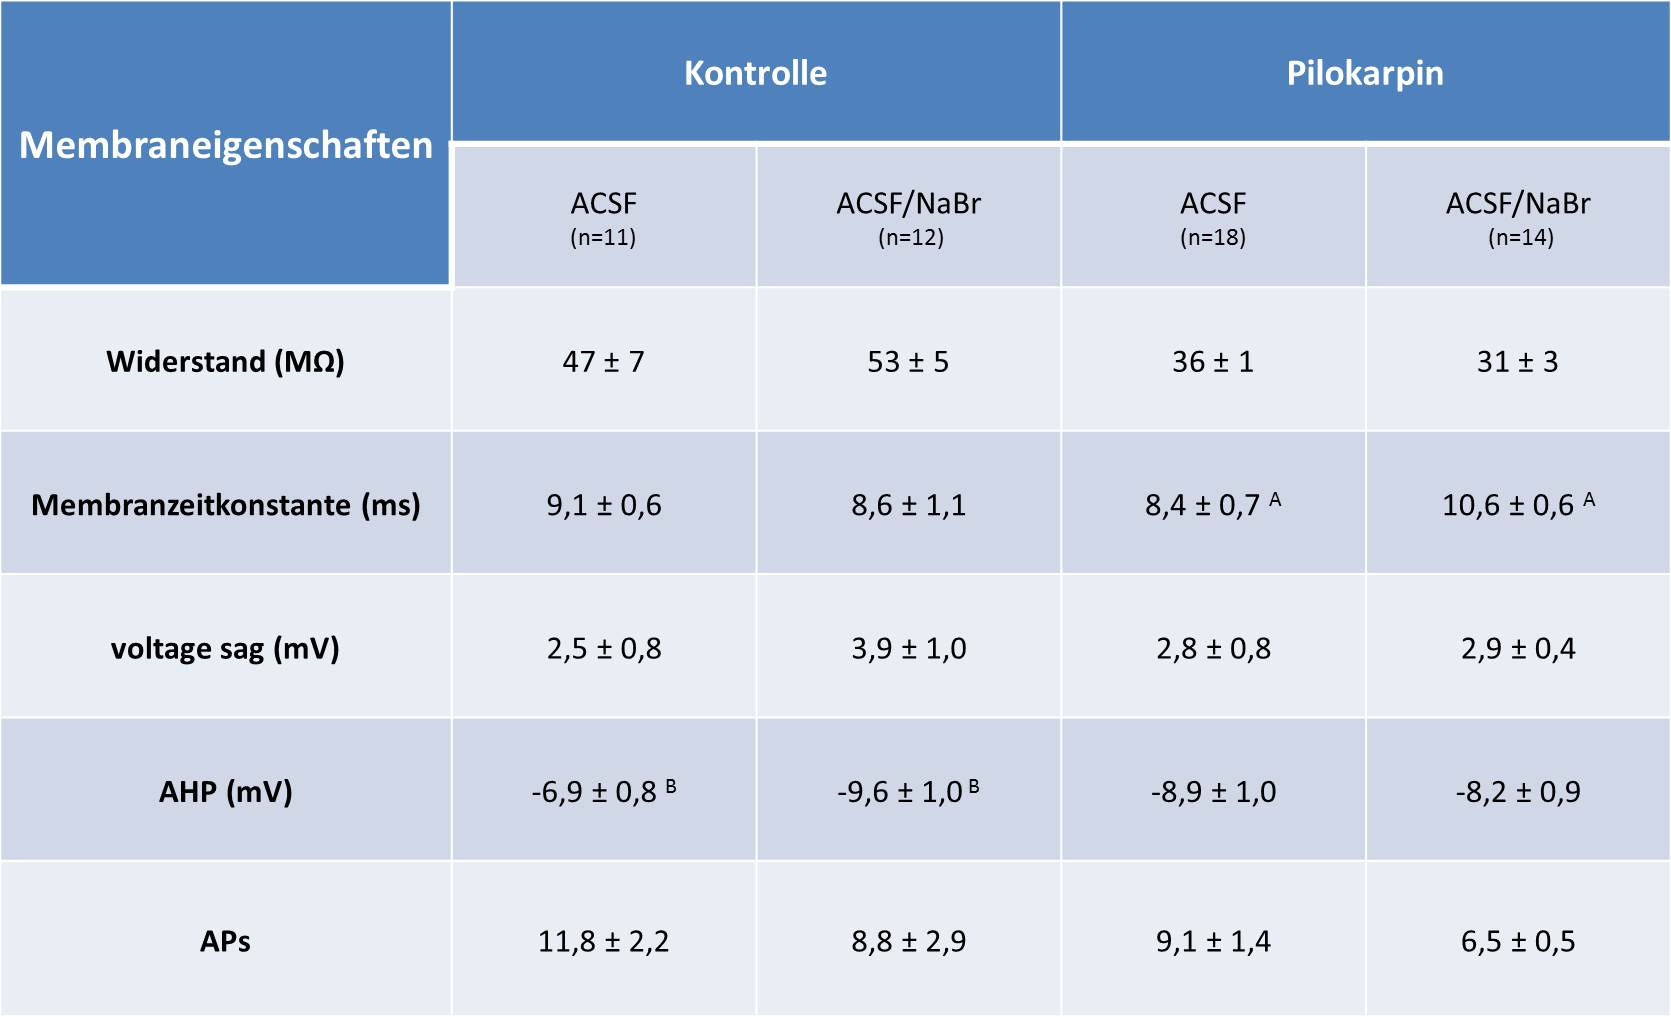
\includegraphics[width= 13cm]{Abbildungen/Membraneigenschaften/tabelle_membraneigenschaften.jpg}
\caption{Dargestellt ist das arithmetische Mittel $\pm$ SEM. Werte, die mit einem gleichen hochgestellten Buchstaben markiert sind, unterscheiden sich voneinander signifikant. Die Werte für den voltage sag, die AHP und die Anzahl der APs sind für eine Stimulation von +1 $nA$ dargestellt}
\end{center}
\end{table}
%Die Messungen ergeben für Kontrolltiere ohne Zugabe von NaBr $9,14 \pm 0,63ms$ für die Membranzeitkonstante. Die Zugabe von NaBr führt zu einem Mittelwert von $8,61 \pm 1,14ms$ und unterscheidet sich damit nicht signifikant vom Kontrollwert.\

Für die Zellen der Pilo-Tiere in Standardlösung ergeben die Messungen eine Membranzeitkonstante mit dem Mittelwert von 8,4$\pm$ 0,7 $ms$.Die Substitution von NaBr erhöht den Mittelwert auf 10,6$\pm$0,6 $ms$.\\

%Für die Zellen der Pilo-Tiere ohne Beigabe von NaBr ergeben die Messungen eine Membranzeitkonstante mit dem Mittelwert von $8,45 \pm 0,71ms$.Die Zugabe von NaBr erhöht den Mittelwert auf $10,65 \pm 0,66ms$
%Für den voltage sag wurden die Werte bei einer Stimulation von $-1nA$ verglichen.
%Bei Kontrolltieren ohne Beigabe von NaBr ergibt sich für den voltage sag ein Mittelwert von $2,50 \pm 0,8 9mV$. Unter Zugabe von NaBr beträgt der Mittelwert $3,92 \pm 1,01 mV$.\

%An Zellen von Pilo-Tieren ohne Beigabe von NaBr beträgt der voltage sag $2,88 \pm 0,84mV$. Der Zusatz von NaBr hat keinen signifikanten Effekt darauf. Es ergibt sich ein Mittelwert von $2,94 \pm 0,41 mV$.\\

Der Mittelwert für das AHP von Kontrolltieren in Abwesenheit von NaBr liegt bei $-6,95 \pm 0,83$ $mV$. Die Substitution von NaBr erniedrigt diesen Wert auf $-9,62 \pm 1,06$ $mV$.\\

In Abbildung 3.4 sind repräsentative Originalregistrierungen des Membranpotentials von Hirnschnitten aller Versuchsgruppen sowohl unter Kontroll- als auch unter Versuchsbedingungen dargestellt. Die verschiedenen Kurven sind durch hyper- und depolarisierende Strominjektionen ausgelöst.

\begin{figure} [H]
\begin{center}

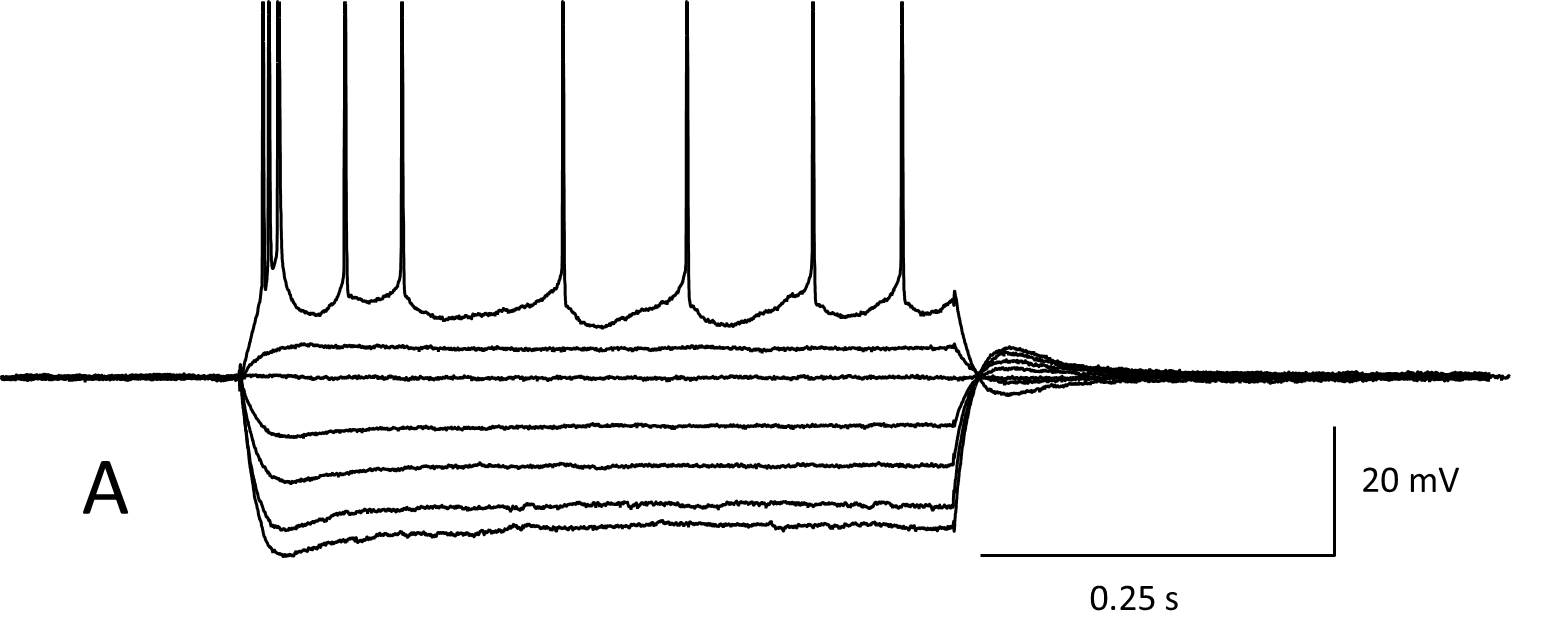
\includegraphics[width=6cm]{Abbildungen/membraneigenschaften/membraneigenschaften_k_c}
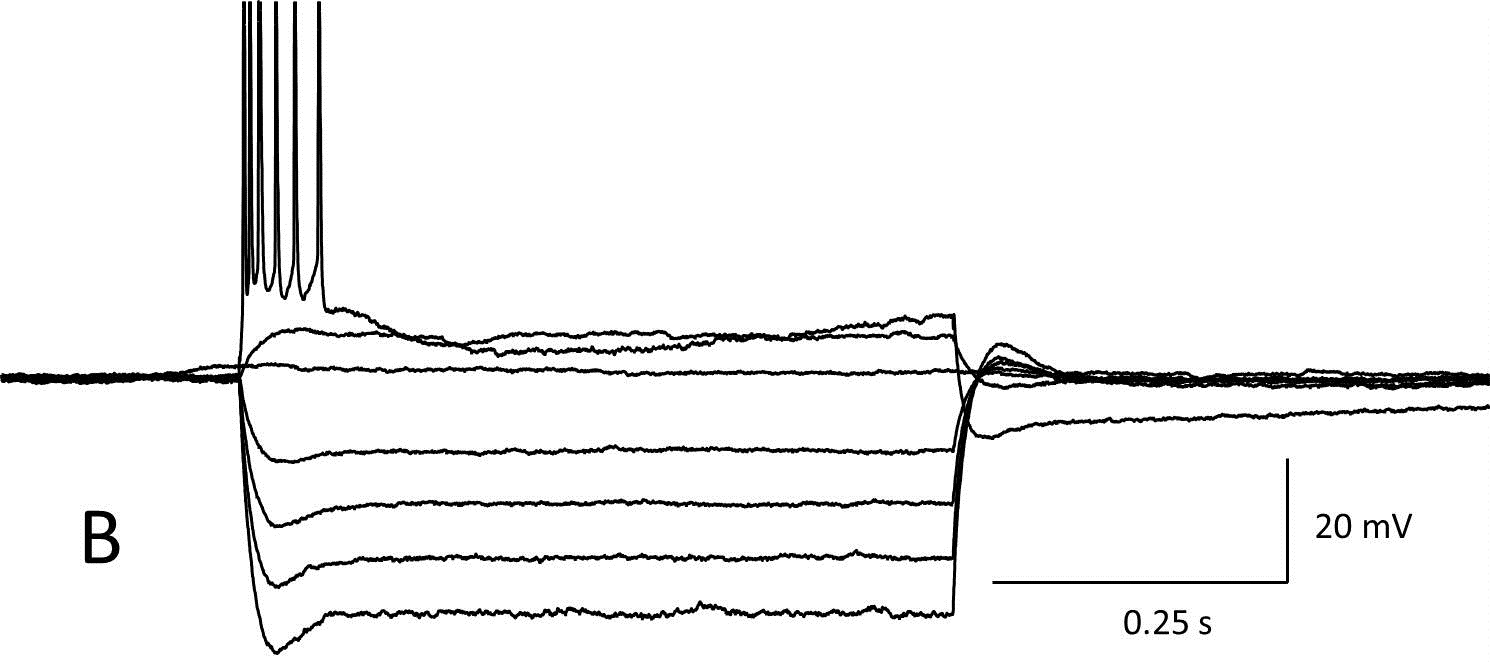
\includegraphics[width=6cm]{Abbildungen/membraneigenschaften/membraneigenschaften_k_br}
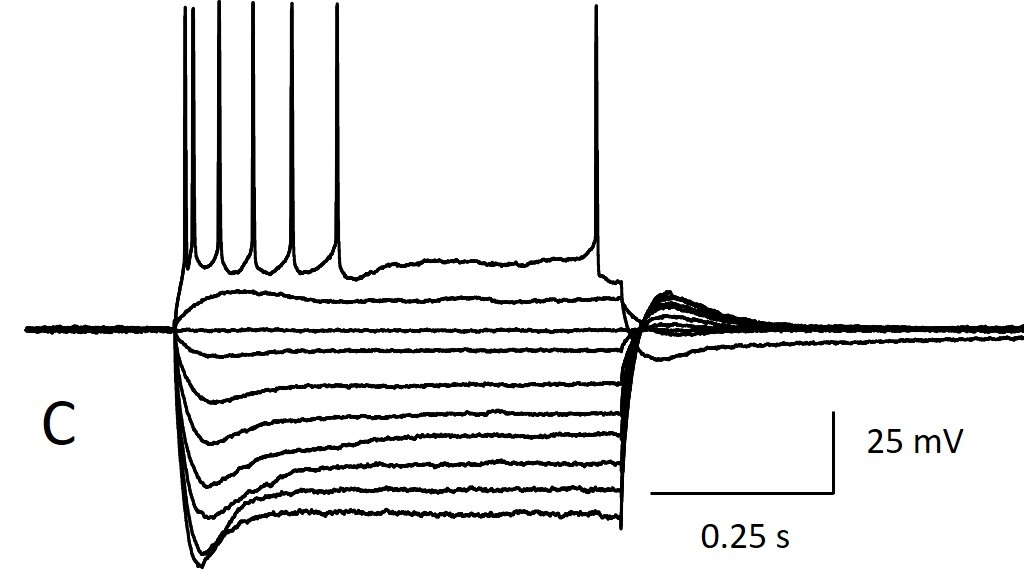
\includegraphics[width=6cm]{Abbildungen/membraneigenschaften/membraneigenschaften_p_c}
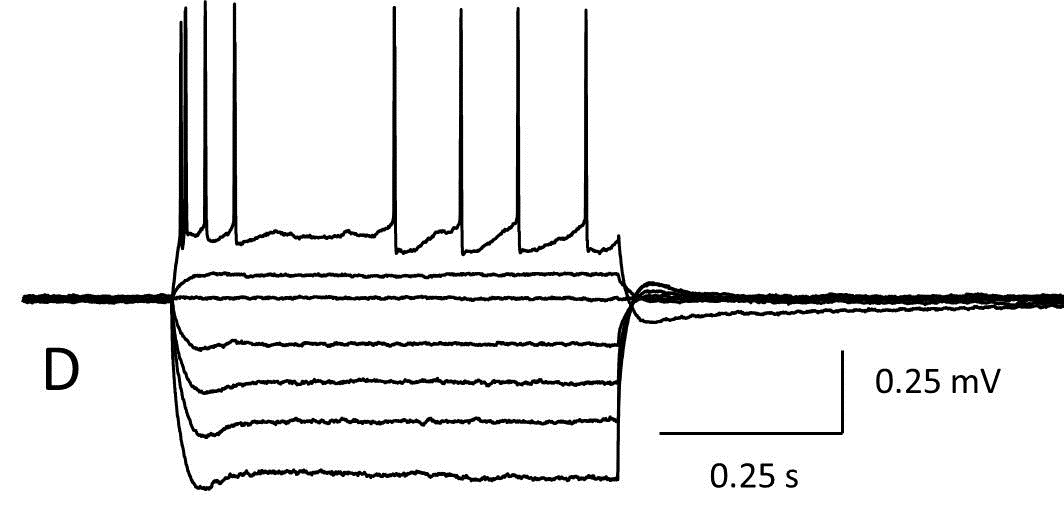
\includegraphics[width=6cm]{Abbildungen/membraneigenschaften/membraneigenschaften_p_br}

\caption{Dargestellt sind repräsentative Originalregistrierungen von Spannungskurven einzelner Zellen aus Hippocampusschnitten. Es erfolgte eine intrazelluläre Strominjektion mit Stromstärken zwischen $-1,3$\,$nA$ und $+1,4$\,$nA$. Zur besseren Übersicht wurden nicht alle Spannungsverläufe dargestellt. Ausgangsniveau jeder Messung ist ein Ruhemembranpotential von $-70\,mV$. Die Kurven \textbf{A} und \textbf{B} repräsentieren Schnitte von unbehandelten Tieren, während die Kurven \textbf{C} und \textbf{D} Schnitte von mit Pilocarpin behandelten Tieren darstellen. Die Schnitte von \textbf{A} und \textbf{C} wurden in herkömmlicher Nährlösung ACSF gemessen. Die Schnitte \textbf{B} und \textbf{D} in modifizierter Nährlösung ACSF/NaBr.}
\end{center}
\end{figure}
%Für Werte der AHP von Zellen von Pilo-Tieren ohne Beigabe von NaBr beträgt der Mittelwert $-8,99 \pm 1,02 mV$. Die Zugabe von Pilokarpin hat keinen signifikanten Einfluss darauf (Mann-Whithney-U-Test). Der neue Erwartungswert liegt bei $-8,27 \pm 0,96 mV$.



%Im Mittel werden an Zellen von Kontrolltieren ohne Beigabe von NaBr bei einer Stimulation von $+1nA$ $11,82 \pm 2,29$ APs ausgelöst. Unter Zugabe von NaBr ändert sich der Erwartungswert nicht signifikant zu $8,82 \pm 2,90$.\
%Die Zellen von Pilo-Tieren weisen bei gleicher Stimulation eine mittlere AP-Entladungsrate von $9,17 \pm 1,40$ auf. Die Zugabe von NaBr senkt die Entladungsrate auf $6,50 \pm 0,54$ (t-Test, p=90).



\section{Stimulations-Antwort-Verhalten hippocampaler Pyramidenzellen}
Um das Stimulus-Antwort-Verhalten zu charakterisieren, wurden die Amplituden der IPSPs gemessen. Es erfolgte eine extrazelluläre Feldstimulation mit steigender Stromstärke zwischen $0,02$\,$mA$ und $0,30$\,$mA$. Nach jeder Stimulation wurde die Stromstärke um $0,02$\,$mA$ erhöht. Die Ableitung der IPSPs erfolgte intrazellulär über scharfe Mikroelektroden. In Abbildung 3.5 sind Beispielkurven jeweils für Messungen an unbehandelten Tieren und mit Pilocarpin behandelten Tieren dargestellt.\\


In Abwesenheit von NaBr unterscheiden sich die Amplituden von Kontrolltieren und Pilo-Tieren nicht signifikant (Two-Way-ANOVA). Der Mittelwert liegt bei Kontrolltieren bei $6,15 \pm 0,85\,mV$ und für Pilo-Tiere bei $5,39 \pm 1,70\,mV$.\\

\begin{figure}[H]
\begin{center}
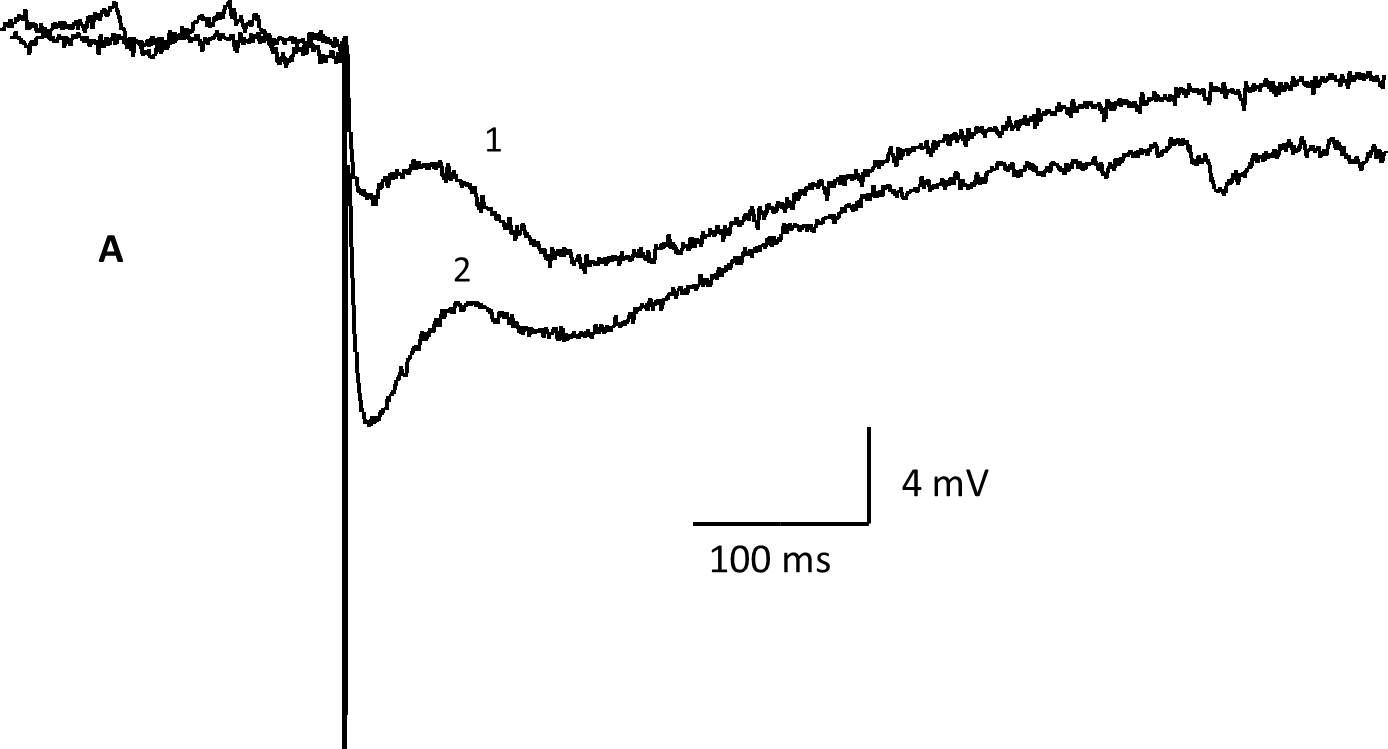
\includegraphics[width=6cm]{Abbildungen/inout_kontrolle_sample.jpg}
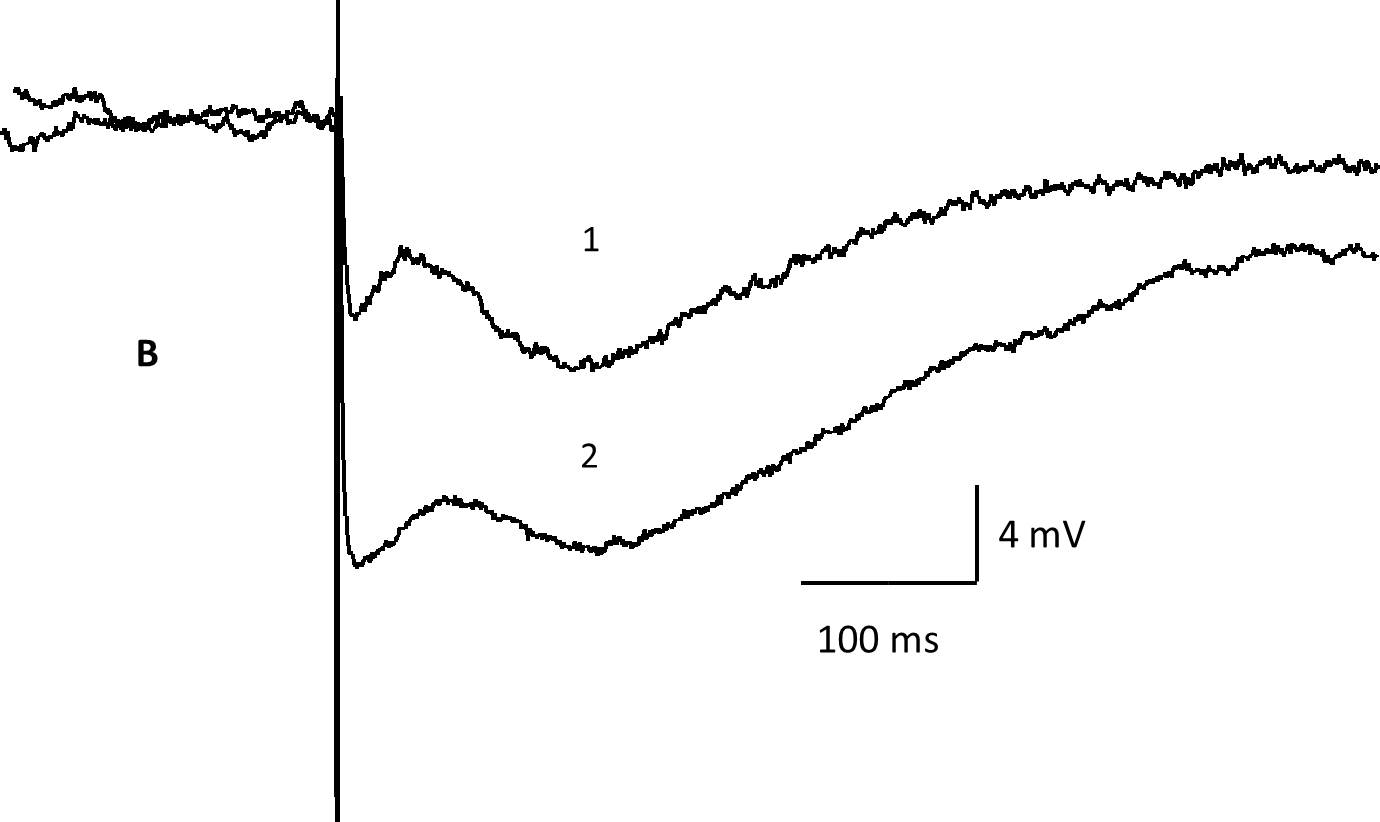
\includegraphics[width=6cm]{Abbildungen/inout_pilo_sample.jpg}
\caption{Dargestellt sind Beispielkurven eines IPSP des Input-Output-Protokolls bei einer Stimulation mit 0.3mA. \textbf{A}  stellt Kurven eines Kontrolltieres dar. \textbf{B} stellt Kurven eines Pilo-Tieres dar. Die mit 1 beschrifteten Verläufe stellen den Versuch in Standardlösung, die mit 2 beschrifteten Verläufe den Versuch unter Substitution mit NaBr dar.}
\end{center}
\end{figure}




Unter Austausch von 20mmol NaCl durch 20mmol NaBr erfolgt bei beiden Versuchsgruppen  eine Steigerung der IPSP-Amplituden. Bei der Kontrollgruppe erhöht sich der Mittelwert auf $9,28 \pm 1,64mV$ (Two-Way-ANOVA).
Bei Pilo-Tieren führt die Substitution mit NaBr zu einer Steigerung der Amplituden auf $13,04 \pm 2,23\, mV$ im Mittelwert (Two-Way-ANOVA). Damit sind unter Versuchsbedingungen die Werte von Zellen von Pilo-Tieren signifikant höher als die Werte der Zellen von Kontrolltieren. \\



\begin{figure}[H]
\begin{center}
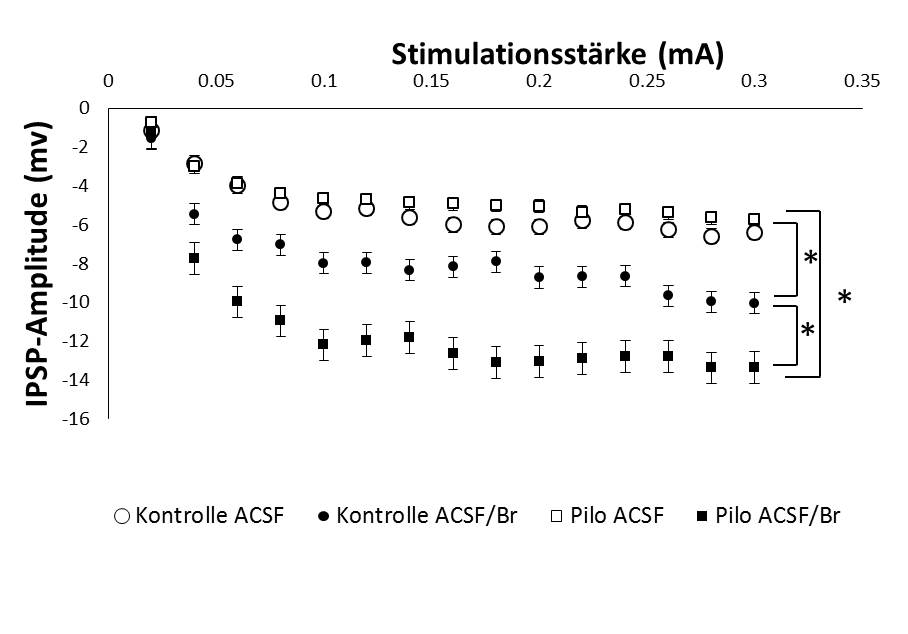
\includegraphics[width=13cm]{Abbildungen/Inout_Diagramm.jpg}
\caption{IPSP-Amplituden in Abhängigkeit der Stimulationsstärke. Um die halbmaximale Stimulationsstärke zu bestimmen wurden Schaffer-Kollateralen in Schritten von $0.02$ $mA$ bis maximal $0.3$ $mA$ stimuliert und die IPSP-Amplituden gemessen. Mit einem Sternchen * markierte Kurven unterscheiden sich voneinander signifikant. }
\end{center}
\end{figure}

Der Test auf Signifikanz erfolgte in allen Gruppen erst ab Stimulationsstärken von $0.6$ $mV$ da bei niedrigeren Stimulationsstärken nicht alle Werte normalverteilt waren, sodass ein Test mit Two-Way-ANOVA nicht möglich war.

Abbildung 3.6 stellt alle Input-Output-Kurven zusammenfassend dar.

\section{Umkehrpotentiale}

Im Anschluss an die Messung der Input-Output-Potentiale wurden bei halbmaximaler IPSP-Amplitude intrazelluläre Strominjektionen von $-0.5\, nA$ bis $0.3\, nA$ durchgeführt und die durch extrazelluläre Feldstimulation ausgelösten IPSPs registriert. Abbildung XX zeigt exemplarische Messungen.\

Die lineare Regression der Werte ermöglicht die Schätzung des Umkehrpotentials des aktivierten Kanals in Form des Schnittpunktes der Regressionsgeraden mit der X-Achse. Die Darstellung der Graphen erfolgt in Abbildung XX.\\

\begin{figure} [H]
\begin{center}
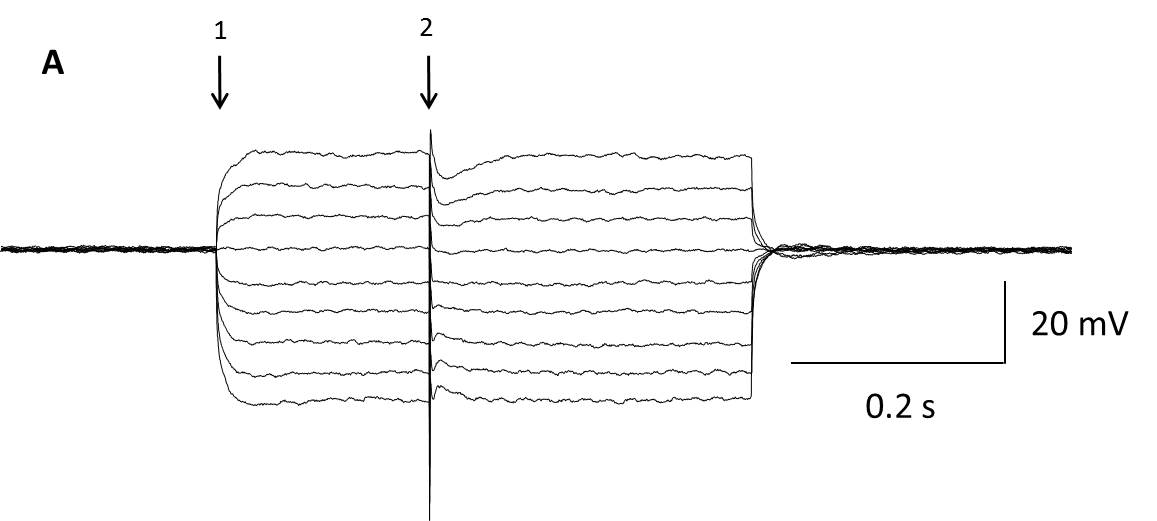
\includegraphics[width=6cm]{Abbildungen/egaba/egaba_k_c_sample}
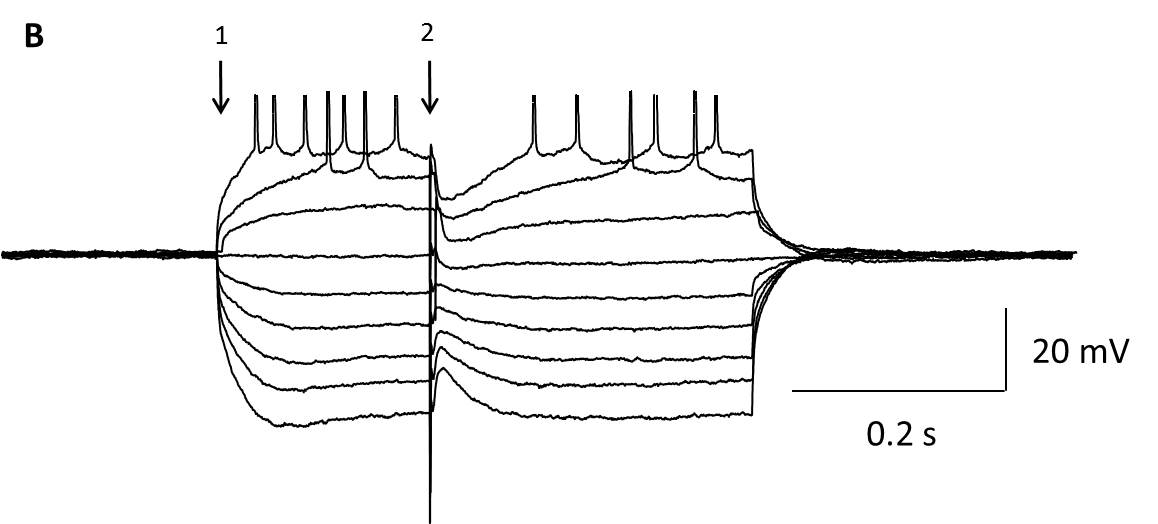
\includegraphics[width=6cm]{Abbildungen/egaba/egaba_k_br_sample}
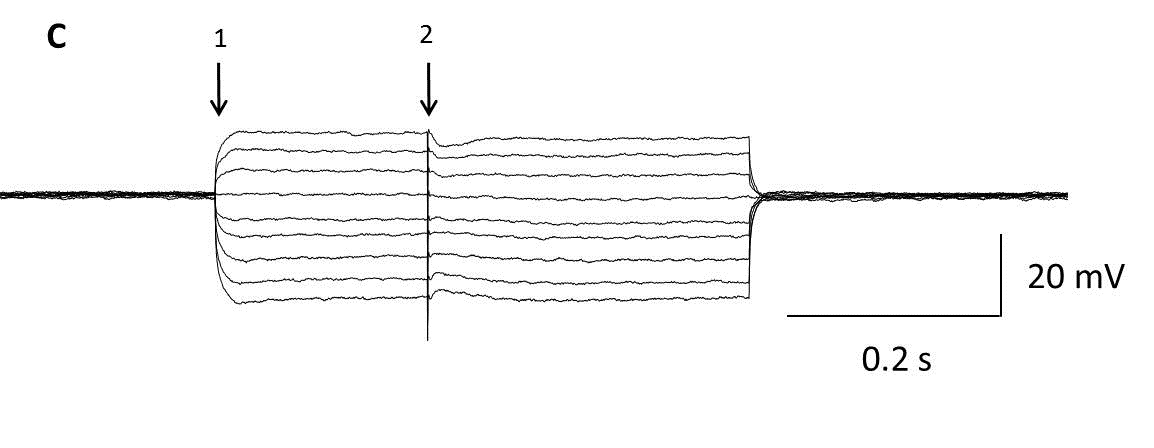
\includegraphics[width=6cm]{Abbildungen/egaba/egaba_p_c_sample}
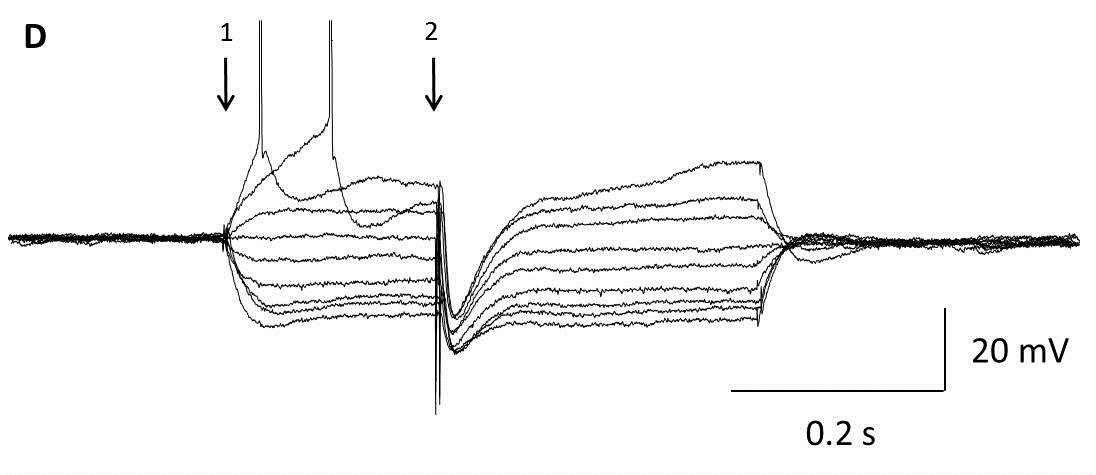
\includegraphics[width=6cm]{Abbildungen/egaba/egaba_p_br_sample}
\caption{Intrazellulär abgeleitete Membranpotentiale. Zum Zeitpunkt 1 erfolgte die intrazelluläre Strominjektion in Höhe von $-0.5\, nA$ bis $0.3$ $nA$. Zum Zeipunkt 2 erfolgte die extrazelluläre Stimulation nahe gelegener Interneurone. Je nach Vorpolarisation und Gruppen- bzw. Behandlungszugehörigkeit lassen sich depolarisierende und hyperpolarisierende Effekte beobachten. \textbf{A} Kontrolltiere ACSF, \textbf{B} Kontrolltiere ACSF/Br, \textbf{C} Pilo-Tiere ACSF, \textbf{D} Pilo-Tiere ACSF/Br.}
\end{center}
\end{figure}

Für die Zellen der Hirnschnitte von Kontrolltieren ergibt sich für die Kontrollgruppe ein Umkehrpotential von $-80,8 \pm 2,4$ $mV$, und für ACSF/Br ein Potential von $-89,2 \pm 4,7$ $mV$. Für Schnitte von Pilo-Tieren beträgt das Potential in ACSF $-84,7 \pm 3,9$ $mV$ und in ACSF/Br $-91,0 \pm 6,8$ $mV$. Ein statistisch signifikanter Unterschied lässt sich nicht nachweisen (Mann-Whithney-Test).

\begin{figure}
\begin{center}
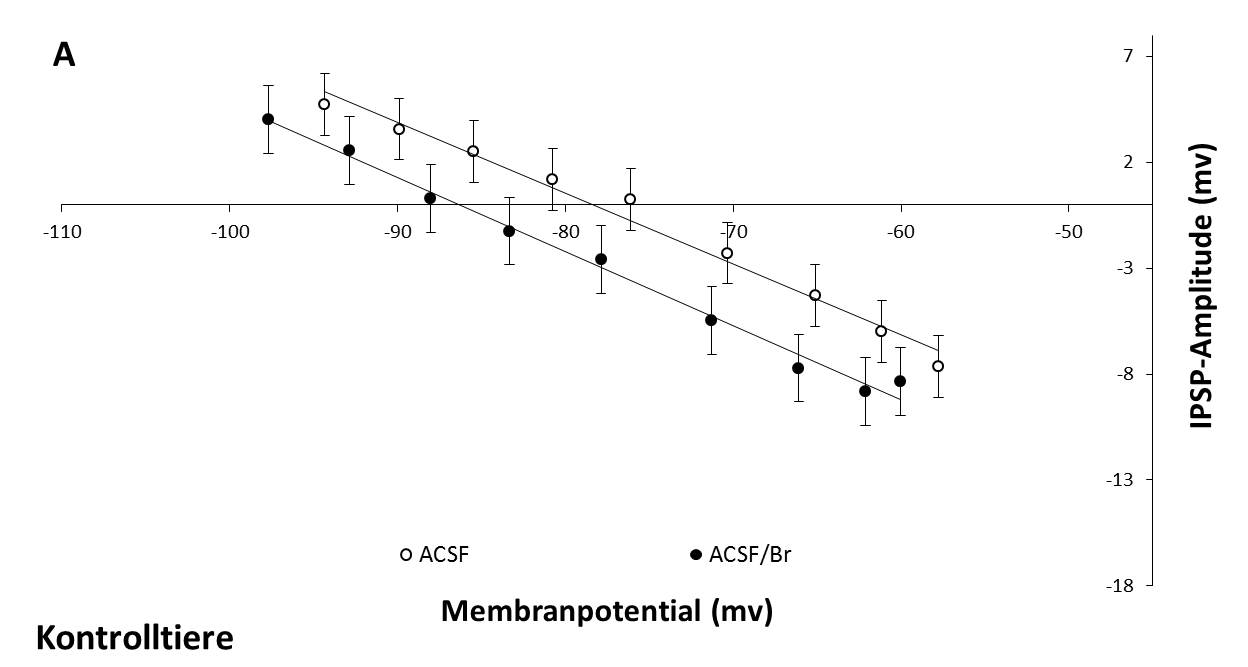
\includegraphics[width=13cm]{Abbildungen/egaba/egaba_kurven_kontrollen}
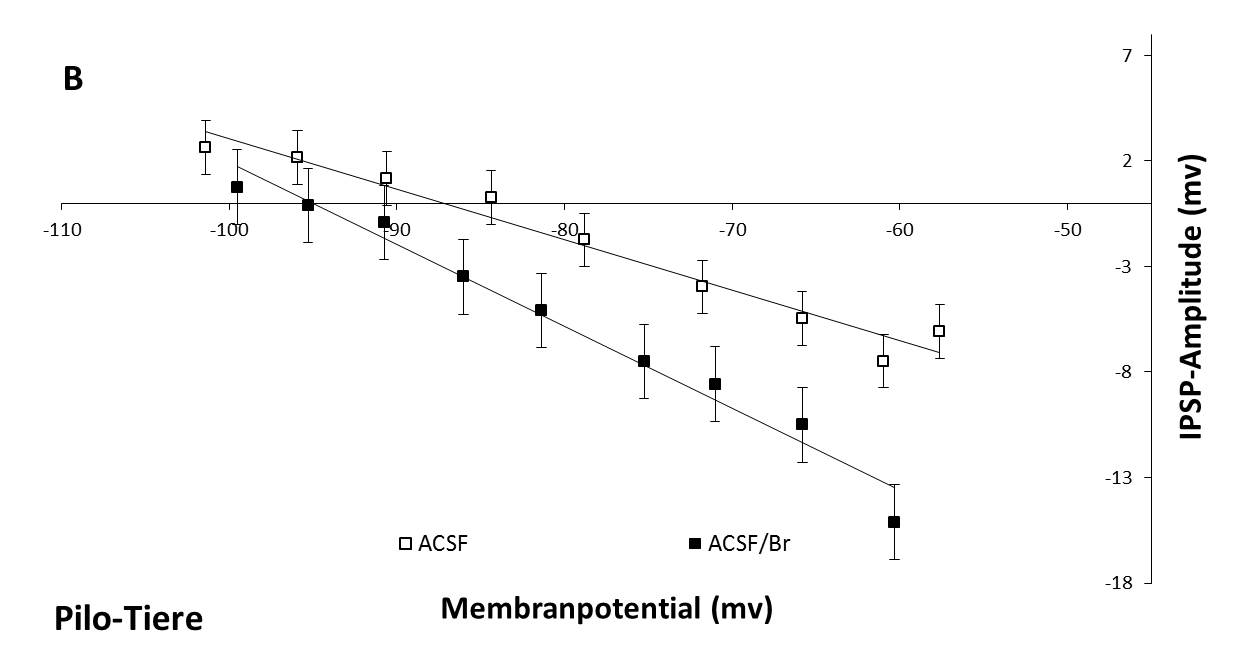
\includegraphics[width=13cm]{Abbildungen/egaba/egaba_kurven_pilo}
\caption{IPSP-Amplituden in Abhängigkeit vom Membranpotential. Positive Werte bedeuten einen negative Ladungsverschiebung des Zellinneren, negative Werte bedeuten eine positive Ladungsverschiebung. Der Schnittpunkt der Regressionsgeraden ist das geschätzte Umkehrpotential des aktivierten Kanals. \textbf{A} zeigt die Werte von Hirnschnitten von Kontrolltieren, \textbf{B} die von Pilo-Tieren.}
\end{center}
\end{figure}








\bibliography{Literaturverzeichnis}{}
\bibliographystyle{plain}

\end{document}
